\documentclass[11pt,reqno]{beamer}
\usepackage[utf8]{inputenc}
\usetheme{Dresden}
\usecolortheme{beaver}

\usepackage[backend=biber, citestyle=authortitle]{biblatex}
\usepackage{amsmath}
\usepackage[normalem]{ulem}
\usepackage{amsfonts}
\usepackage{mhchem}
\usepackage{array}
\usepackage{graphicx}
\usepackage{tabularx}
\usepackage{hyphenat}

\addbibresource{references.bib}
\setbeamertemplate{navigation symbols}{}
%BondGraphTools: Modelling network bioenergetics.
%
%Energy is the currency of physical systems, yet models of biological processes often neglect to account for energy and power. While this is not necessarily a problem when describing an individual process, capturing the flow of energy is crucial for building systems level models that avoiding pathological behavior such as perpetual motion. Following how energy is transformed also allows for increasingly physical descriptions of multi-domain processes such as cellular respiration (electro-chemical) and muscular contraction (electro-chemo-kinetic).
%
%In many interesting cases, metabolism for example, cellular systems can be described using a network topology. These networks describe how energy is transformed from one form or location to another. It is this network topology that allows one to talk about distinct subnetworks (the Krebb cycle, for example) and conceptually organize a system into ‘modules’.
%
%Here we present a new software library ‘BondGraphTools’ that allows scientists and engineers to programmatically build and simulate networked models of energy systems. Implemented in Python and Julia, ‘BondGraphTools’ is designed to be intuitive and easy to use whilst providing the efficacy of a modern CAD. We demonstrate some interesting and useful applications of ‘BondGraphTools’ for modelling cross-domain cellular processes.


\title{BondGraphTools: Modelling Network Bioenergetics}
\author{Peter Cudmore}
\titlegraphic{
\begin{columns}
	\begin{column}{0.4\textwidth}
		\centering
		\includegraphics[height=1.5cm]{cbns-logo}
	\end{column}
	\begin{column}{0.5\textwidth}
		\centering
		\includegraphics[width=1.75cm]{PRIMARY_A_Vertical_Housed_RGB.png}
	\end{column}
\end{columns}
}
\subtitle{https://github.com/peter-cudmore/}
\date{}

\graphicspath{{../images/}{.}}

\newcommand{\D}[2]{\frac{\mathrm{d} #1}{\mathrm{d} #2}}
\newcommand{\e}{\mathrm{e}}
\newcommand{\I}{\mathrm{i}}
\renewcommand{\mod}[1]{\left|#1\right|}
\newcommand{\DD}[2]{\frac{\mathrm{d}^2 #1}{\mathrm{d} #2^2}}
\newcommand{\bigO}[1]{\text{O}\left(#1\right)}
\renewcommand{\P}[2]{\frac{\partial #1}{\partial #2}}
\renewcommand{\Re}{\operatorname{Re}}
\renewcommand{\Im}{\operatorname{Im}}
\newcommand{\EX}{\mathbb{E}}
\newcommand{\df}[1]{\mspace{2mu}  \mathrm{d}#1}
\newcommand{\reals}{\mathbb{R}}
\newcommand{\complex}{\mathbb{C}}
\newcommand{\conj}[1]{\overline{#1}}

\newcommand{\fcite}[1]{
\footnote{\tiny\cite{#1}, (\citeyear{#1}).}
}
\newcommand{\fciteauthor}[1]{\citeauthor{#1}\fcite{#1}}
\setbeamercolor{block body}{fg=black, bg=red!10 }
\setbeamertemplate{block begin}{
	\vskip.75ex
	\begin{beamercolorbox}[rounded=true,leftskip=1cm,colsep*=.75ex]{block title}%
		\usebeamerfont*{block title}\insertblocktitle
	\end{beamercolorbox}%
	{\ifbeamercolorempty[bg]{block body}{}{\nointerlineskip\vskip-0.5pt}}%
	\usebeamerfont{block body}%
	\begin{beamercolorbox}[rounded=true, colsep*=.75ex,sep=.75ex,vmode]{block body}%
		\ifbeamercolorempty[bg]{block body}{\vskip-.25ex}{\vskip-.75ex}\vbox{}%
	}

\setbeamertemplate{block end}{\end{beamercolorbox}
}


\AtBeginSection[] { 
	\begin{frame}
	\tableofcontents[currentsection,hideallsubsections] 
	\addtocounter{framenumber}{-1} 
\end{frame}
}
\begin{document}
\begin{frame}
\titlepage
\addtocounter{framenumber}{-1} 
\end{frame}
% Basics of biochemical processes
\section{Modelling Biochemical Systems}
\begin{frame}{An Example Biochemical Systems.}
\begin{figure}
\includegraphics[width=0.8\linewidth]{map.png}
\caption{Map of the Human Metabolome\fcite{HMDB}}
\end{figure}
\end{frame}

\begin{frame}{Biochemical systems are complex.}
We want to:
\begin{itemize}
	\item Predict how particular \emph{nonequilibrium} states depend upon system parameters and network topology.
	\item Track how these states vary with parameter changes.
	\item Design and implement synthetic control devices.
\end{itemize}
\vspace{20pt}

\emph{We require models that can be used to engineer biological systems!}
\end{frame}

\begin{frame}{Problems At Scale.}
Issues that can occur when attempting to `scale-up' existing approaches:
\begin{itemize}
	\item<2-> \emph{Models may not generalise}.
	\item<3-> \emph{Models may not integrate}.
	\item<4-> \emph{Models may not be parametrisable}.
\end{itemize}
\vfill
\only<2>{Models may not capture the environment, and hence fail to predict how a process behaves in different circumstance. For example; \emph{in vitro} vs \emph{in vivo}.}
\only<3>{Models may fail to correctly describe shared physical quantities, such as two different processes known to sharing the same enzyme, and hence incorrectly infer modularity.}
\only<4>{Even if there did exist a sufficient amount of observational data, certain parameters may not be inferable, let alone observable.}
\end{frame}

\begin{frame}{Problem: Non-physical models}
The Michaelis-Menten `law' for enzyme dynamics:
\begin{columns}
	\begin{column}{0.45\linewidth}
		\ce{E + S <=> ES -> E + P}
	\end{column}
	\begin{column}{0.45\linewidth}
		\[
		\D{[P]}{t}= - \D{[S]}{t} = \frac{V_\text{max}[S]}{[S] + K_m}
		\]
	\end{column}
\end{columns}
\vfill

\begin{block}{}
	\begin{quote}
		...in model building [the Michaelis-Menten approximation] is often invoked without regard to the underlying assumptions.\fcite{Keener2009}
	\end{quote}
\end{block}
\end{frame}
\begin{frame}{Problem: Retroactivity\fcite{DelVecchio2013}}
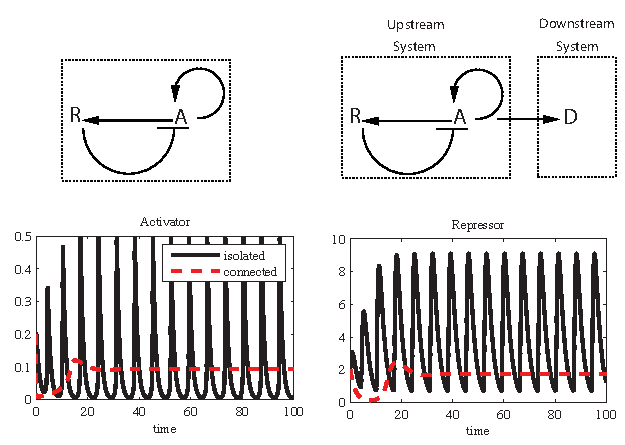
\includegraphics[height=6cm]{activator-repressor-ddv}
\end{frame}

\begin{frame}{Problem: 'Sloppy' Parameters}
\begin{block}{}
\begin{quote}`Sloppy' is the term used to describe a class of complex models exhibiting large
parameter uncertainty when fit to data.\fcite{Transtrum2015}
\end{quote}

\end{block}

\vfill

For example, fitting decaying observations $y(t)$ to
\[
y(t;\theta) = \sum_\mu \exp(-\theta_\mu t) 
\]
\begin{center}
\emph{Each parameter $\theta_\mu$ is almost completely undetermined.}\\
\emph{Data {\bf constrains} parameters!}
\end{center}
\end{frame}
\begin{frame}{Problems At Scale.}
Question: How do we address the fact that
\begin{itemize}
	\item \emph{models may not generalise},
	\item \emph{models may not integrate},
	\item \emph{models may not be parametrisable}.
\end{itemize}
\vfill
\pause
Answer (or at least, one approach): \emph{Network Energetics}.
\end{frame}

\section{Network Energetics}

\begin{frame}
\frametitle{The Fundamental Law: Conservation of Energy}
\begin{quotation}
There is a fact, or if you wish, a law, governing all natural phenomena that are known to date. There is no known exception to this law—it is exact so far as we know.
The law is called the conservation of energy.
\end{quotation}

\vspace{10pt}
- Richard Feynman, 1963\fcite{Feynman1963}.
\end{frame}

\begin{frame}
\frametitle{Bond Graphs}
Bond Graphs\fcite{Paynter2000} are a graphical representation of how energy networks distribute power through a physical system.

\begin{minipage}{0.45\linewidth}
\includegraphics[width=\linewidth, height=0.66\linewidth]{hydro.jpg}
\end{minipage}
\begin{minipage}{0.45\linewidth}
	
\begin{itemize}
	\item Energy is currency
	\item Discrete subsystems
	\item Power flows via ports
\end{itemize}
\end{minipage}

\emph{Network thermodynamics}\fcite{Oster1971} and \emph{port Hamiltonians}\fcite{VanderSchaft2014b} followed.  
\end{frame}
\begin{frame}
\frametitle{Bond Graph of \ce{A + B <=> C}}
\begin{figure}
	\includegraphics{bondgraph_abc_naive}
\end{figure}
\begin{itemize}
	\item `Ce' nodes \emph{store energy} (via concentration)
	\item The `Re' node \emph{dissipate energy}
	\item The `1' node is a conservation law. (Conservation of flow)
	\item $e$ is `pressure'-like (similarly force or voltage).
	\item $f$ is `flow'-like (similarly velocity, or current).
	\item $P_i = e_i\times f_i$ is the instantaneous power $P_i = \D{}{t}\text{energy}_i$ 
\end{itemize}
\end{frame}
\begin{frame}
\frametitle{Chemical Subsystems Store Energy}
\begin{minipage}{0.35\linewidth}
	\includegraphics[width=\linewidth]{oneport-Ce}
\end{minipage}
\begin{minipage}{0.55\linewidth}
\begin{align*}
e &= \mu^\oslash(R,T) + RT\ln\left(\frac{n}{c^\oslash V}\right),\\
f &=\dot{n}.
\end{align*}
\end{minipage}
\vfill
\only<1>{
This is just a network reformulation of the Gibbs free energy $\df{G} = V\df{p} - S\df{T} + \mu\df{n}$ for
\begin{itemize}
\item constant pressure $p = R$
\item constant temperature $T$
\item constant volume $V$
\item Reference concentration $c^\oslash$ and chemical potential $\mu^\oslash$ 	
\end{itemize}
}
\only<2-5>{
\begin{center}
	\only<2>{$\mu^\oslash$ has controlled dependence on the environment.}
	\only<3>{$\mu^\oslash$ can be estimated and (occasionally) measured.}
	\only<4>{$\mu^\oslash$ is taken as a derived physical quantity of that molecule.}
	\only<5>{$\mu^\oslash$ is supposed to generalise across experimental conditions.}
\end{center}}
\end{frame}

\begin{frame}
\frametitle{Chemical Reactions Dissipate Energy}
\begin{minipage}{0.45\linewidth}
	\includegraphics[width=\linewidth]{twoport-Re}
\end{minipage}
\begin{minipage}{0.45\linewidth}
	\begin{align*}
	f_1 &= \kappa\left[\e^{e_1/RT} - \e^{e_2/RT}
	\right],\\
	0 &= f_1 + f_2.
	\end{align*}
\end{minipage}
\vfill
\only<1>{
This is a network reformulation of the Marcelin de-Donder formula, which relates reaction affinities $e_1, e_2$ to the flow $f_1 = -f_2$.
}

\only<2-5>{
\begin{center}
	\only<2>{$\kappa$ is a constant relating time and extent of reaction}
	\only<3>{$\kappa$ is not generally measurable!}
	\only<4>{$\kappa$ is constant for simple reactions}
	\only<5>{$\kappa$ can be a function for more complex models. \\
		For example; $\kappa = (\alpha + \beta\exp(e_1))^{-1}$ can produce a Hill equation.
}
\end{center}}
\end{frame}
\begin{frame}
\frametitle{Bond Graph of \ce{A + B <=> C}}
\begin{figure}
	\includegraphics{bondgraph_abc_naive}
\end{figure}
If we define $k_i = \frac{1}{Vc^\oslash_i}\exp(\mu^\oslash_i/RT)$; evaluating the model
\[
f_i = \dot{C} = - \dot{A} = - \dot{B} =  \kappa \left(k_Ak_B AB - k_C C \right) = k_+AB - k_CC
\] 
with
\[
k_+ = \kappa k_Ak_b,\quad  k_- =\kappa k_C, \qquad  k_\text{Eq} =k_Ak_B/k_C.
\]

\end{frame}
\begin{frame}
\frametitle{How does Network Energetics help?}
\begin{itemize}
\item Based on well established physics.
\item Processes and parameters are tied to physical properties. 
\item Power connections by definition capture 'loading effects'.
\item Parameters can be fitted across many experiments.
\end{itemize}
\vfill

This gives us a framework to predict, engineer and refine \emph{reusable} models of processes.
\end{frame}

\begin{frame}
\frametitle{Trade offs}
Bond Graphs/Network Energetics:
\begin{itemize}
	\item<1-> is more complicated than doing it by hand\\
	\emph{but it can be done algorithmically}.
	\item<2-> is more `abstract' than some other modelling techniques\\
	\emph{but it can handle multi-physics}.
	\item<3-> fitting a particular experiment even more difficult\\
	\emph{but parameters can be tabulated}.
\end{itemize}
\end{frame}
\section{BondGraphTools}
\begin{frame}
\frametitle{BondGraphTools}
\vfill
BondGraphTools
\begin{itemize}
	\item is a Python library for network energetics model building,
	\item has addons specifically for biological processes,
	\item is designed to be used alongside and in conjunction with scipy,
	\item is symbolic yet has simulation tools
\end{itemize}
\end{frame}
\section{Conclusion}
\begin{frame}
For more information on BondGraphTools visit \url{bondgraphtools.readthedocs.io}
\vfill
Thanks to:
\begin{itemize}
	\item Prof. Edmund Crampin, Prof. Peter Gawthrop \& the Systems Biology Lab, The University of Melbourne.
	\item The Australian Research Council Center of Excellence for Convergent Bio-nano Science (CBNS).
	\item ANZIAM 2019 and Victoria University.
	\item The session chair, and you.
\end{itemize}


\end{frame}
\begin{frame}[allowframebreaks]
\tiny
\printbibliography
\end{frame}

\end{document}
